\chapter{Surrogate Modelling}

\section{Physics-Constrained Neural Networks}
By definition, NNs are designed to reproduce their training data in a best possible manner, defined by the characteristics of the loss
function used during the training process. NN predictions minimize the loss towards the training data seen beforehand.
Circumstances exist, in which the output of a NN should strictly satisfy a certain set of equations. In case of
physical modeling, the prediction of a surrogate should follow the same conservation laws as a first principle model. Especcialy,
when predicions are propagated through several NNs or simulated in an autoregressive manner, errors accumulate. 
Final predictions are untrustworthy or simulations exhibit instability \cite{chen2024}. As a MPC algorithm needs a reasonable
approximation of the system behavior over the complete prediction horizon, the accumulation of conservation violations
become an issue.
\newline
\newline
To realize physics consistent NN outputs, several strategies exists. Physics-informed neural networks (\emph{PINN}s) for instance,
embed physical balance equations into the loss function similar to a regularization term \cite{raissi2019}. This serves as a 
soft constraint and comes with two downsides.
The NN output does not strictly follow the constraint equation, because the physical consistency is fullfilled up to
the trade off between data fit and constraint satisfaction.
Every new balance equation to be included introduces a new hyperparameter worsening the ability to include network parameter regularization.
To guarantee strict constraint satisfaction and thus perfect physics consistency up to machine precision,
a new type of activation function is presented equivalently to the work by Chen et al. \cite{chen2024}. This activation function serves as a linear projection from the NN output space
into the physical allowed subspace without adding neither learnable parameters nor hyperparameters.
Let the output of a NN be defined as well as a set of linear equality contraints that summarize some physical conservation quantity (def.~\ref{def: physics consistency}).


\begin{definition} Crude NN output with a given set of linear equality constraints.
    \label{def: physics consistency}
    \[
        \begin{gathered}
        \bm{\tilde{y}}(\bm{\theta}, \bm{\xi}) \coloneq \mathcal{NN}(\bm{\theta}, \bm{\xi})
        \\
        \bm{A} (\bm{y} - \bm{z}_0) = \bm{b}
        \\
        \text{with}
        \quad
        \bm{\tilde{y}}(\bm{\theta}, \bm{\xi}), \bm{z}_0 \in \mathbb{R}^{n_\text{out}}
        \quad
        \bm{A} \in \mathbb{R}^{n_\text{c} \times n_\text{out}}
        \quad
        \bm{b} \in \mathbb{R}^{n_{\text{c}}}
        \end{gathered}
    \]
\end{definition}


$\bm{\tilde{y}}$ denotes the NN output, $\bm{\xi}$ the input and the matrices $\bm{A}$ and $\bm{b}$ portray the feasible space of points.
The variable $\bm{z}_0$ illustrates an external input into the constraint. This may be a NN input, a constant, or another batched 
reference point. In a physical sense, $\bm{z}_0$ is often introduced as a boundary or initial condition.
A feasible point $\bm{y}$ now needs to be determined that fullfills the set of linear equality constraints.
For a straight forward implementation, the formulation appears in such a way that it supports batching of 
a certain batch size $n_\mathcal{B}$. $n_\text{out}$ and $n_\text{c}$ describe the number of output features and numbers
of linear equality constraints respectively. The main idea is, to find a point in the feasible subspace that is closest to the NN prediction. This is 
forced by following quadratic programm (QP) (def.~\ref{def: physics constrained optimization}).

\begin{definition} Minimization of the euclidian distance towards the NN output as a linear equality constrained optimization that supports batching.
    \label{def: physics constrained optimization}
    \[
        \begin{aligned}
            \bm{y}^* = \underset{\bm{y}}{\mathrm{argmin}} || \bm{y} - \bm{\tilde{y}} ||_2^2 
            \\
            \mathrm{s.t.} \quad (\bm{y} - \bm{z}_0) \bm{A}^\top - \bm{b} = \bm{0}
        \end{aligned}
    \]
\end{definition}
This means, the output of the network $\bm{\tilde{y}}$, the optimal solution $\bm{y}^*$ and $\bm{z}_0$ are matrices of
dimension $n_\mathcal{B}~\times~n_\text{out}$. Computing frameworks that support broadcasting such as \texttt{numpy} or
\texttt{pytorch} allow the implementation of $\bm{z}_0$ in the shape of $1 \times n_\text{out}$ to reduce memory usage as long as it remains constant \cite{empty000}.
The transposed constraint matrix $\bm{A}^\top$ must be of shape
$n_\text{c}~\times~n_\mathcal{B}$. The vector $\bm{b}$ represents the offset of the linear equality constraints. This optimization
task can be solved analytically by setting up the \emph{Karush-Kuhn-Tucker} (KKT) conditions (th.~\ref{th: physics constrained KKT}).

\begin{theorem} Langrangian and KKT conditions of the QP
    \label{th: physics constrained KKT}
    \[
        \begin{aligned}
            \mathcal{L}(\bm{y}, \bm{\nu}) &= ||\bm{y} - \bm{\tilde{y}}||_2^2 + \bm{\nu}^\top (\bm{A}(\bm{y}-\bm{z}_0)^\top - \bm{b})
            \\
            \nabla_{\bm{y}} \mathcal{L}(\bm{y}, \bm{\nu}) &= 2(\bm{y}^*-\bm{\tilde{y}}) + \bm{\nu}^\top \bm{A} \overset{!}{=} 0
            \\
            \nabla_{\bm{\nu}} \mathcal{L}(\bm{y}, \bm{\nu}) &= (\bm{y}^* - \bm{z}_0) \bm{A}^\top - \bm{b} \overset{!}{=} 0
        \end{aligned}
    \]
\end{theorem}

The Lagrangian $\mathcal{L}$ arises as the sum of the objective function and all linear equality constraints.
The vector $\bm{\nu}$ contains the dual variables of the linear equality constraints.
The optimality conditions lead to a linear system of equations (cor.~\ref{cor: physics constrained solution}).


\begin{corollary} The optimal solution in the feasible space as projection of an activation function
    \label{cor: physics constrained solution}
    \begin{gather*}
    \begin{pmatrix} \bm{y}^* & (\bm{\nu}^*)^\top \end{pmatrix}
    \begin{pmatrix}
        2 \bm{I} & \bm{A}^\top  \\
        \bm{A} & \bm{0}   
    \end{pmatrix} = 
    \begin{pmatrix} 2 \bm{\tilde{y}} & \bm{z}_0 \bm{A}^\top + \bm{b} \end{pmatrix}
    \\
    g_\text{pc}(\bm{\tilde{y}}, \bm{z}_0) \coloneq
    \begin{pmatrix} 2 \bm{\tilde{y}} & \bm{z}_0 \bm{A}^\top + \bm{b} \end{pmatrix}
        \begin{pmatrix}
        2 \bm{I} & \bm{A}^\top  \\
        \bm{A} & \bm{0}   
    \end{pmatrix} ^{-1} 
    = \begin{pmatrix} \bm{y}^* & (\bm{\nu}^*)^\top \end{pmatrix}
\end{gather*}
\end{corollary}

The optimal solution denoted with "*" is directly yielded by projecting the NN output $\bm{\tilde{y}}$
using the additional input $\bm{z}_0$ and a projection matrix. This projection matrix only contains the constraint matrix $\bm{A}$ can be computed
before runtime which drastically speeds up forward and backward passes in contrast to implicit methods \cite{cvxpylayers2019}.
The solution elegantly serves as an 
activation function $g_\text{pc}(\bm{\tilde{y}}, \bm{z}_0)$, that maps the crude NN output into a subspace defined by $\bm{A}$ and $\bm{b}$. The final output
for $\bm{y}^*$ satisfies the linear equality constraints by definition, while it is located as close to the crude
output $\bm{\tilde{y}}$ as possible. 
This is not only applicable in the field of chemical engineering but a 
general formulation that allows to integrate linear equality constraints into NNs.
Additionally, the type of network architecture is independent of the mapping. It can be appended to any 
network type such as recurrent NNs, convolutional NNs or transformer-based architectures.
\newline

\begin{figure}
    \centering
    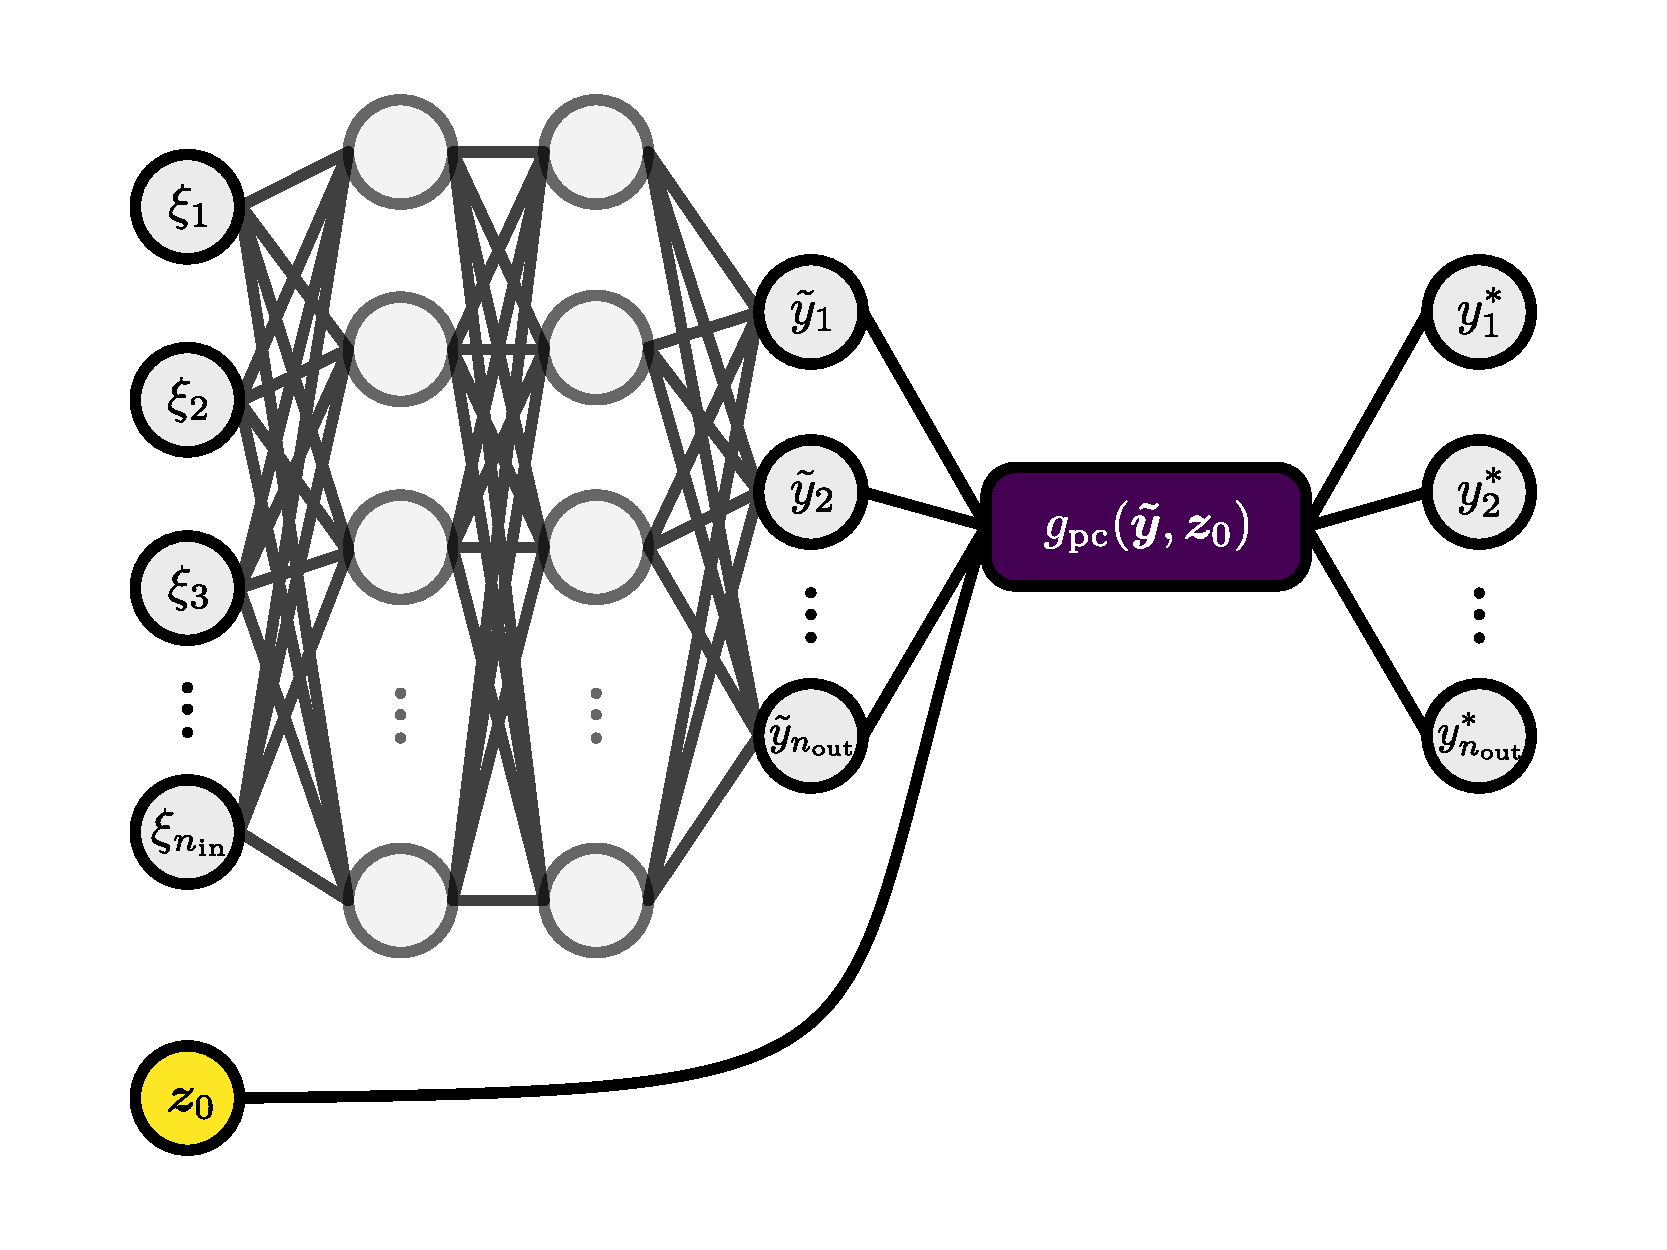
\includegraphics[width=1\textwidth]{Figures/Theory/pc_neural_network.pdf}
    \caption[Neural network with physics constrained activation function $g_\text{pc}$]
    {The physics constrained NN turns the input vector $\bm{\xi}$ into the crude output $\bm{\tilde{y}}$ via
    a feedforward NN, which is the projected by the physics constrained activation function $g_\text{pc}$
    into the feasible output $\bm{y}^*$. It allows to include data points such as boundary conditions as needed in the form of $\bm{z}_0$}
    \label{theory:fig: pc_neural_network}
\end{figure}

Due to its general applicability, the activation function could be used within a network to correct intermediate values.
In most use cases howerver, it is applied as a final correction function at the output (fig.~\ref{theory:fig: pc_neural_network}).
The input $\bm{\xi}$ is propagated through a feedforward NN with the physics constrained activation function behind the last layer (purple).
It takes the reference value $\bm{z}_0$ (yellow) without beeing forwarded through the network.
In recent literature, NNs that utilze such a
type of activation function can be found as \emph{KKT-hPINN}~\cite{chen2024}, which is short 
for \emph{Karush-Kuhn-Tucker-hard-physics-informed-neural-network}.
For later reference, this activation function $g_\text{pc}$ will be referred to as \emph{physics constrained activation} (cor.~\ref{cor: physics constrained solution}) to have
a short name in the context of chemical engineering. 
Furthermore, this procedure could be extended
to support arbitrary non-linear equality constraints by splitting the network output in frozen and unfrozen variables~\cite{lastrucci2025}.
It enables the integration of enthalpy balances that are of non-linear nature. As this work combines the implementation
of physics consistent NNs with parametric uncertainty for MPC, the focus remains on linear equality constraints.

\begin{algorithm}
	\caption{Forward pass of the physics constrained activation function.}
	\label{theory:algo: pc forward pass}
	\begin{algorithmic}
		\REQUIRE $\bm{K} = 
            \begin{pmatrix}
                2 \bm{I} & \bm{A}^\top  \\
                \bm{A} & \bm{0}   
            \end{pmatrix} ^{-1} $,
                $\bm{\tilde{y}}, \vz_{0}, \bm{A}, \bm{b}$
		\STATE $\bm{h} \leftarrow 
            \begin{pmatrix}
                2 \bm{\tilde{y}} & \bm{z}_0 \bm{A}^\top + \vb
            \end{pmatrix}$
        \STATE $\bm{y}^* \leftarrow \vh \bm{K}$
        \STATE $\bm{y}^* \leftarrow $ $\bm{y}^*_{:,:n_\text{out}}$
        \RETURN $\bm{y}^*$
	\end{algorithmic}
\end{algorithm}

The forward pass through the physics constrained activation involves the setup of a temporary vector $\vh$ (alg.~\ref{theory:algo: pc forward pass})
and the truncation of the dual variables in the solution. The matrix inversion to yield $\bm{K}$ should be done 
offline and then saved as untrainable model parameter. In \texttt{pytorch} this is can be done using the
\texttt{register\_buffer()} method. An implementation example of the physics consistent activation can be found in the appendix (XX).

